\section{Конструкторский раздел}
В данном разделе будут приведены схемы рассмотренных в предыдущем разделе алгоритмов сортировки и произведен расчет их трудоемкости.

\subsection{Разработка алгоритмов}

На рисунках  \ref{fig:sorting-bubble}, \ref{fig:sorting-insertion} и \ref{fig:sorting-bucket} представлены схемы алгоритмов сортировки пузырьком, вставками и блочной соответственно.
\clearpage

\begin{figure}[h!btp]
	\centering
	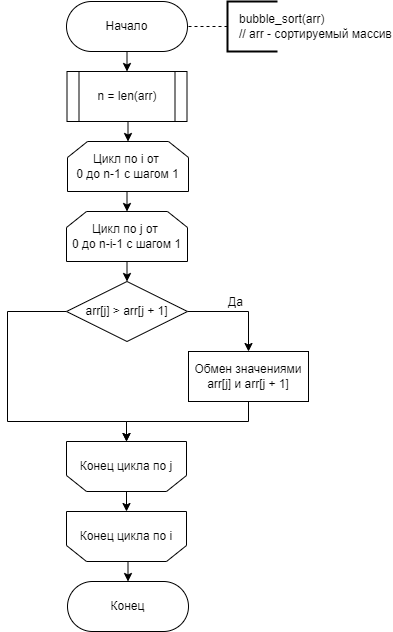
\includegraphics[width=310pt]{inc/sorting-bubble.png}
	\caption{Схема алгоритма сортировки пузырьком}
	\label{fig:sorting-bubble}	
\end{figure}
\clearpage

\begin{figure}[h!btp]
	\centering
	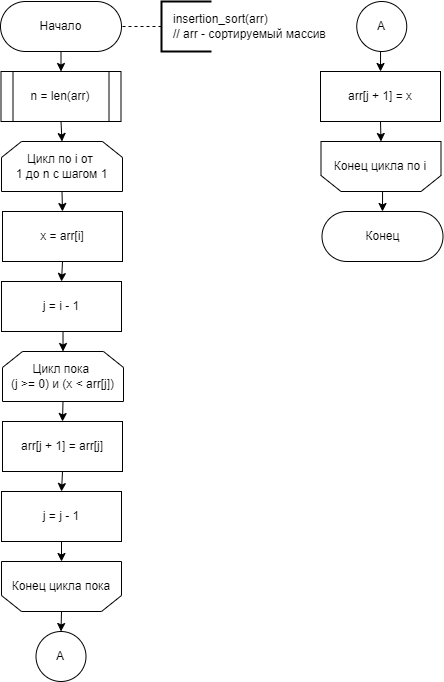
\includegraphics[width=340pt]{inc/sorting-insertion.png}
	\caption{Схема алгоритма сортировки вставками}
	\label{fig:sorting-insertion}	
\end{figure}
\clearpage

\begin{figure}[h!btp]
	\centering
	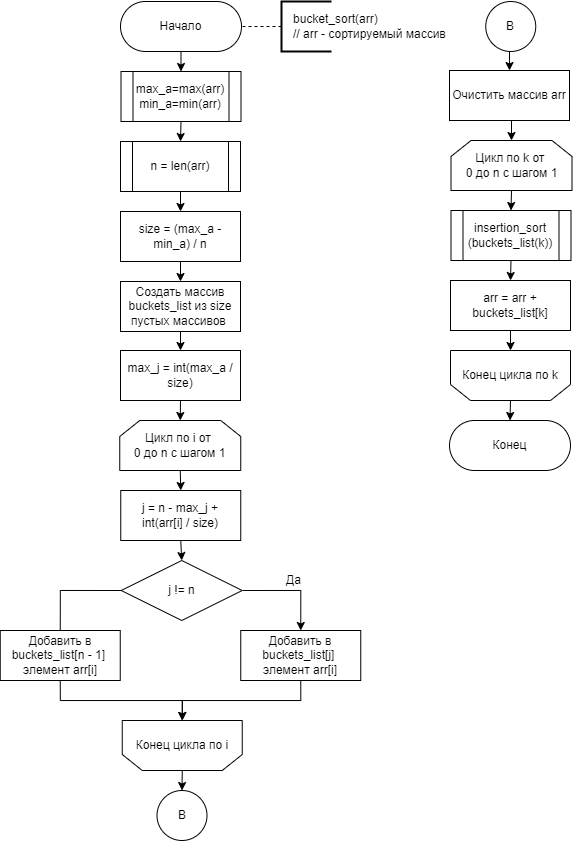
\includegraphics[width=420pt]{inc/sorting-bucket.png}
	\caption{Схема алгоритма блочной сортировки}
	\label{fig:sorting-bucket}	
\end{figure}
\clearpage

\subsection{Оценка трудоемкости}

Для последующего вычисления трудоемкости необходимо ввести модель вычислений.

\begin{enumerate}

	\item Трудоемкость следующих базовых операций единична:
	+, -, =, +=, -=, ==, !=, <, >, <=, >=, [], ++, --, <<, >>.
	
	Операции *, \%, / имеют трудоемкость 2.
	
	\item Трудоемкость цикла for(k = 0; k < N; k++) \{тело цикла\} рассчитывается как
	\begin{equation}
		\label{for:for}
		f_{for} = f_{\text{инициал.}} + f_{\text{сравн.}} + N(f_{\text{тела}} + f_{\text{инкр.}} + f_{\text{сравн.}})
	\end{equation}
	
	\item Трудоемкость условного оператора \code{if (условие) then A else B} рассчитывается как
	
	\begin{equation}
		\label{for:if}
		f_{if} = f_{\text{условия}} +
		\begin{cases}
			min(f_A, f_B), & \text{в лучшем случае;}\\
			max(f_A, f_B), & \text{в худшем случае.}
		\end{cases}
	\end{equation}
	
\end{enumerate}


\subsubsection{Сортировка пузырьком}

\textbf{Лучший случай:} массив отсортирован (ни одного захода в тело условного оператора).\newline
$f = 1 + 2 + (n - 1)(1 + 2 + 1 + 3) + \frac{n(n - 1)}{2}(4 + 4 + 0) = 4n^2 + 3n - 4 = O(n^2) $

\textbf{Худший случай:}  массив отсортирован в обратном порядке (на каждой итерации заход в тело условного оператора).\newline
$f = 1 + 2 + (n - 1)(1 + 2 + 1 + 3) + \frac{n(n - 1)}{2}(4 + 4 + 7) = \frac{15}{2}n^2 - \frac{1}{2}n - 4 = O(n^2) $


\subsubsection{Сортировка вставками}

\textbf{Лучший случай:} массив отсортирован (ни одного захода во внутренний цикл).\newline
$f = 1 + 2 + (n - 1)(1 + 2 + (2 + 1 + 4 + 0 + 2)) = 12n - 9 = O(n) $

\textbf{Худший случай:}  массив отсортирован в обратном порядке (на каждой итерации заход во внутренний цикл).\newline
$f = 1 + 2 + (n - 1)(1 + 2 + (2 + 1 + 4 + 2) + \frac{1}{2}n(n - 1)(4 + 5)) = \frac{9}{2}n^2 + \frac{15}{2}n - 9 = O(n^2) $


\subsubsection{Блочная сортировка}

\textbf{Лучший случай:} массив отсортирован, элементы распределены равномерно (все блоки содержат одинаковое число элементов).\newline
$f = 7 + 3 + n(1 + 1) + 3 + 2 + n(1 + 1 + 5 + 2) + 1 + 2 + n(1 + 1 + 1 + 12size - 9 + 3) = 8n + 12n + 18 = 20n + 18 = O(n) $

\textbf{Худший случай:} элементы распределены неравномерно (большое количество пустых блоков), массив отсортирован в обратном порядке (худший случай сортировки вставками, которая используется в блочной сортировке).\newline
$f = 7 + 3 + n(1 + 1) + 3 + 2 + n(1 + 1 + 5 + 3) + 1 + 2 + n(1 + 1 + 3) + \frac{9}{2}(n - 1)^2 + \frac{15}{2}(n - 1) - 9 - 9 = \frac{9}{2}n^2 + \frac{31}{2}n - 3 = O(n^2) $


\subsection*{Вывод}

Были разработаны схемы трех алгоритмов сортировки, определены лучшие и худшие случаи, а также произведен расчет трудоемкости алгоритмов.